\documentclass[a4paper]{article}
\usepackage{fullpage} % Package to use full page
\usepackage{parskip} % Package to tweak paragraph skipping
\usepackage{amsmath}

\usepackage{float}
\usepackage{tikz}
\usepackage{xfrac}
\usepackage[outdir=./Plots]{epstopdf}
\usepackage{pgfplots}
\usepackage{graphicx}    
\usepackage{caption}
\usepackage{mathtools}
\usepackage{comment}
\usepackage{gensymb}
\usepackage{textcomp}
\usepackage{xcolor}
\usepackage{hyperref}

\usepackage{tikz}
\usetikzlibrary{shapes,arrows}
\usetikzlibrary{arrows,calc,positioning}

\tikzset{
	block/.style = {draw, rectangle,
		minimum height=1cm,
		minimum width=2cm},
	input/.style = {coordinate,node distance=1cm},
	output/.style = {coordinate,node distance=4cm},
	arrow/.style={draw, -latex,node distance=2cm},
	pinstyle/.style = {pin edge={latex-, black,node distance=2cm}},
	sum/.style = {draw, circle, node distance=1cm},
}

\usepackage{subcaption}
\setlength{\parindent}{1em}
\graphicspath{{./Images/}}
\title{ATI Mini40 DAQ F/T sensor information and tips}
\author{Iris David Du Mutel}

\begin{document}
	
\maketitle

\begin{abstract}
	This document is meant to be a summary of all the relevant information I have found while working with the ATI Mini40 DAQ F/T sensor. It contain all the information and instructions to operate such sensor in various environments such as LabView, Python and MATLAB using the Keysight 34970A Data Acquisition Unit. 
\end{abstract}


\section{What kind of sensor is the ATI Mini40 DAQ F/T}

\section{Wiring and connecting to a DAQ}

\subsection{Sampling}

\section{Keysight 34970A connection to PC}
The connection is made via a GPIB‑USB‑HS cable. The GPIB‑USB‑HS is an IEEE 488 controller device for computers with USB slots. The GPIB‑USB‑HS achieves maximum IEEE 488.2 performance. The exact model can be found in \hyperref{https://www.amazon.com/Kanonaki-GPIB-USB-HS-Interface-Adapter-Controller/dp/B07Q84XJJF}{category}{name}{Amazon}. The differences with the \hyperref{https://www.newark.com/ni/780570-01/gpib-usb-hs-gpib-control-device/dp/14AJ5119}{category}{name}{original} true version of this device are not the sxope of this document. 


\section{LabView}

LabView offers two main ways of interacting with the Keysight 34970A DAQ:

\begin{itemize}
	\item General purpose Virtual Instrument Software Architecture (VISA) blocks.NI-VISA is an API that provides a programming interface to control Ethernet/LXI, GPIB, serial, USB, PXI, and VXI instruments in NI application development environments like LabVIEW, LabWindows/CVI, and Measurement Studio. The API is installed through the NI-VISA driver \cite{NIVISA}.
	\item Agilent Technologies / Keysight Technologies 34970A \hyperref{http://sine.ni.com/apps/utf8/niid_web_display.model_page?p_model_id=5547}{category}{name}{drivers}. These block are based on the VISA blocks but offer a more user-friendly approach to configuring the instrument as well as reading data from it. 
\end{itemize}

The \hyperref{https://github.com/IrisDuMutel/ATIMini40_software/tree/master/LabView}{cat1}{visa}{example}  provided in this repository uses generic VISA blocks. In \autoref{fig:labview_block}, the block diagram of the VI can be seen:

\begin{figure}[!h]
	\centering
	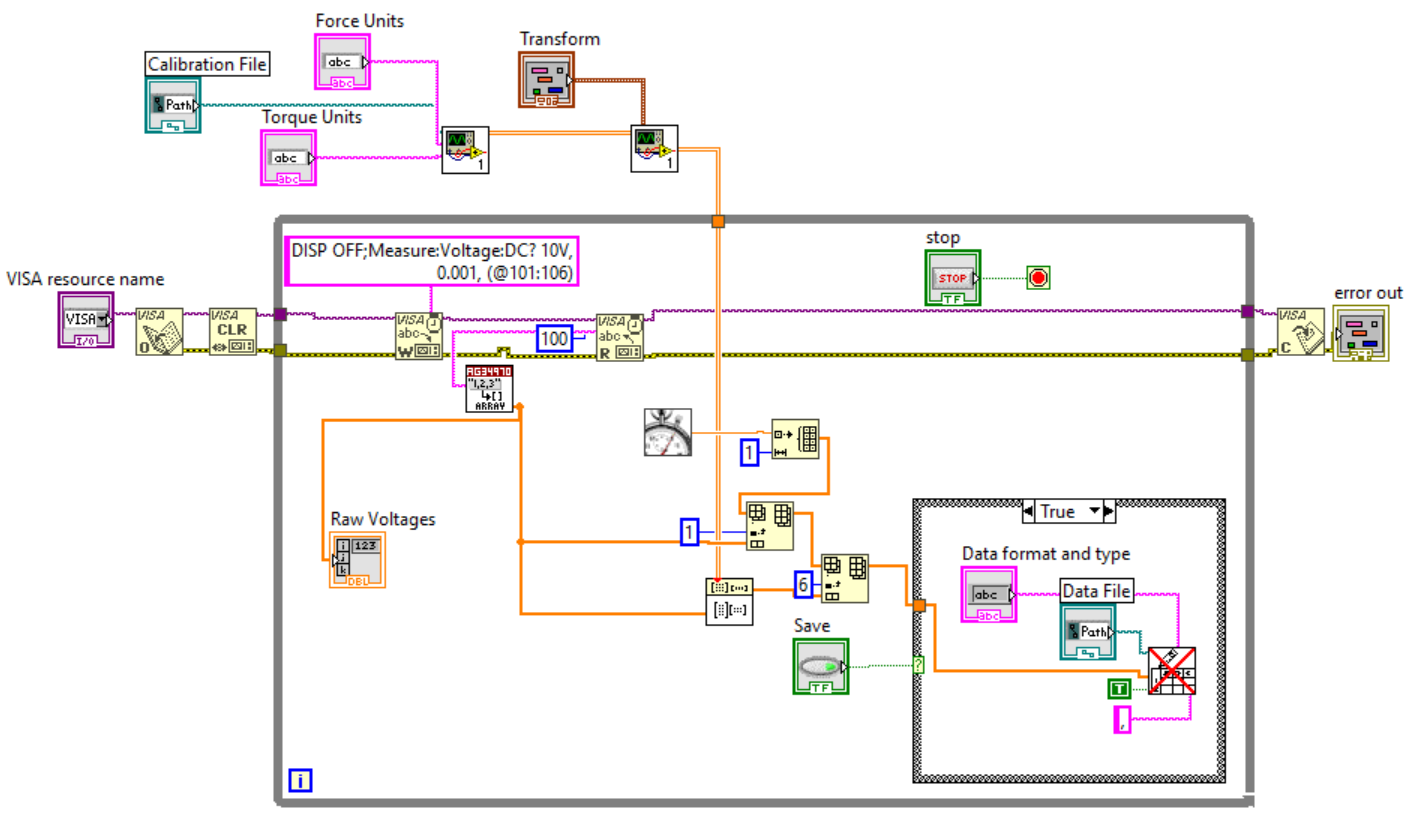
\includegraphics[width=0.9\textwidth]{labview_block.png}
	\caption{LabView block diagram}
	\label{fig:labview_block}
\end{figure}

Inside the while loop, the write and read blocks are interacting with the instrument. Every iteration, the \textit{write} block sends the following commands to the DAQ:

\begin{itemize}
	\item DISP OFF: This command turns off the display of the external instrument. This speeds up the sampling process.
	\item MEASure:VOLTage:DC? 10V, 0.001, (@101:106): The first part of the command 'MEASure:VOLTage:DC$?$` is requesting the measurement of the voltage. The question mark indicates a query command. The two numbers following such query are the \textit{range} and the \textit{resolution}, respectively. There are alternative values for these parameters. See more in pages 211 to 217 from the \hyperref{https://www.manualsbase.com/manual/439362/switch/hp_(hewlett-packard)/hp_34970a/}{category}{name}{manual}.
\end{itemize}

\section{Python}



\bibliographystyle{IEEEtran}
\bibliography{biblio}

\end{document}
